\documentclass[100,a4paperpaper,]{article}

  \title{\textbf{\textcolor{white}{Relatório de Conjuntura}}}
  \author{\textbf{\textcolor{white}{Crédito}}}
  \date{\textbf{\textcolor{white}{Outubro/2021}}}
  


\newcommand{\logo}{c:/Users/700105212/R Projects/econdashboard/inst/app/www/img/logo-banestes-transparente.png}
\newcommand{\cover}{c:/Users/700105212/R Projects/econdashboard/inst/app/www/img/cover-banestes-menor.png}
\newcommand{\logotitle}{c:/Users/700105212/R Projects/econdashboard/inst/app/www/img/logo-banestes-branca.png}
\newcommand{\iblue}{004b8d}
\newcommand{\igray}{d4dbde}
\usepackage{booktabs}
\usepackage{longtable}
\usepackage{array}
\usepackage{multirow}
\usepackage{wrapfig}
\usepackage{float}
\usepackage{colortbl}
\usepackage{pdflscape}
\usepackage{tabu}
\usepackage{threeparttable}
\usepackage{threeparttablex}
\usepackage[normalem]{ulem}
\usepackage{makecell}
\usepackage{xcolor}

% Author: Karol KozioL
% License: GPL-3
% Modified by: Sarah Wagner

% % % packages -----------------------------------------------------------------------------------
\usepackage{amsmath}
\usepackage{array}
\usepackage{booktabs}
\usepackage{calc}
\usepackage{eso-pic}
\usepackage[left = 30pt, right = 30pt, top = 25pt, bottom = 25pt, headsep = 40pt, includeheadfoot]{geometry}
\usepackage{fancyhdr}
\usepackage{fontspec}
\usepackage{graphicx}
\usepackage[utf8]{inputenc}
\usepackage{lastpage}
\usepackage{multirow}
\usepackage{tabularx} 
\usepackage{tikz}
\usepackage{titlesec}
\usepackage{titling}
\usepackage{xcolor, colortbl}
\usepackage{etoolbox}
\usepackage{ragged2e}
\usepackage{xcolor}
\usepackage[fontsize=14]{scrextend}
\usepackage[portuguese]{babel}
\usepackage{indentfirst}

% % % settings -----------------------------------------------------------------------------------

% % custom colors
\definecolor{iblue}{HTML}{\iblue}
\definecolor{igray}{HTML}{\igray}

% definition of pagename
\newcommand\pagename{Page}

% % fonts 
\defaultfontfeatures{Mapping = tex-text}
\setmainfont{Arial}
\newfontfamily\headingfont{Arial}



% % sections
\titleformat{\section}{\color{iblue}\headingfont\Large\bfseries}{\thesection}{1em}{}[\titlerule]
\titleformat{\subsection}{\color{iblue}\headingfont\large\bfseries}{\thesubsection}{1em}{}
\titleformat{\subsubsection}{\color{iblue}\headingfont\large\bfseries}{\thesubsubsection}{1em}{}

% % misc
\setlength{\parindent}{0em} 
\setlength{\parskip}{1em}
\linespread{1.15}
\renewcommand{\baselinestretch}{1.25}
\raggedright
\newcolumntype{C}{>{\centering\arraybackslash}X}
\justifying


% % % custom titlepage ----------------------------------------------------------------------------
\newcommand\BackgroundPic{%
	\put(0,0){%
		\parbox[b][\paperheight]{\paperwidth}{%
			\vfill
			\centering
			
\includegraphics[width=\paperwidth,height=\paperheight]{\cover}%
			\vfill
}}}

\makeatletter

% pagestyle titlepage
\fancypagestyle{customtitle}{
	\lhead{}
	\chead{}
	\rhead{\includegraphics{\logotitle}}
	\makeatother
	\lfoot{}
	\cfoot{}
	\rfoot{}
}


% titlepage
\renewcommand{\maketitle}{
	\thispagestyle{customtitle}
	\AddToShipoutPicture*{\BackgroundPic}
	\ClearShipoutPicture
	
	\phantom{a}\hfill
	\vspace{12cm}
	
	\begin{tabular}[l]{@{}p{\textwidth}@{}}
		\color{iblue}\headingfont\LARGE\@title\\[1em]
		\color{iblue}\headingfont\Large\@author\\[1em]
		\color{iblue}\headingfont\large\@date\\[1em]
	\end{tabular}
	
	
	\clearpage
}

\makeatother

% % % header and footer ---------------------------------------------------------------------------
\pagestyle{fancy}
\lhead{}
\chead{}
\rhead{ 
\includegraphics{\logo}}
\makeatother
\newlength{\myheight}
\lfoot{}
\cfoot{}
\rfoot{\pagename~\thepage \hspace{1pt} / \pageref{LastPage}}
\renewcommand\headrulewidth{0pt}
\renewcommand\footrulewidth{0pt}




\begin{document}


\renewcommand{\contentsname}{Sumário}


\maketitle
\tableofcontents
\clearpage

\section{Operações de crédito do Sistema Financeiro Nacional (SFN)} 
 \vspace{0.5cm}

De acordo com o Banco Central, o saldo total de crédito cresceu 18,8\%
no acumulado dos últimos doze meses. Apesar do aumento, o índice de
inadimplência se mantém estável em 2,3\% desde maio deste ano.

Nesse sentido, é preciso ter cautela na avalição destes dados, uma vez
que o Comitê de Política Monetária (COPOM), na tentativa de conter o
avanço da inflação, mantém uma trajetória de alta da taxa básica de
juros (SELIC), atualmente em 9,25\%.

É fundamental observar os dados macroeconômicos, uma vez que, a Selic
impacta diretamente a taxa de juros das novas operações de crédito do
Sistema Financeiro Nacional, a taxa de juros das operações de crédito
atingiu 23,2\% a.a. em outubro, com elevação de 1,5\% em relação ao mês
anterior e de 4,6\% no acumulado em doze meses.

O spread bancário, diferença entre as taxas de aplicação e captação,
atingiu 15,3\% com alta mensal de 0,7\% e de 0,8\% no acumulado em doze
meses.

Nas operações de crédito com recursos livres (com taxas de juros
livremente pactuadas entre mutuários e instituições financeiras) a taxa
média de juros situou-se 32,8\% a.a. em outubro, com variação de 2,2\%
no mês e de 6,3\% em comparação ao mesmo período do ano anterior.

No crédito livre destinado às pessoas jurídicas, a taxa média de juros
atingiu 19,1\% a.a. e para pessoas físicas atingiu 43,8\% a.a., com
aumentos de 2,1 p.p. no mês e de 4,8 p.p. em 12 meses.

\newpage

\section{Saldo das operações} 
 \vspace{0,25cm}

O saldo total de empréstimos no Sistema Financeiro Nacional (SFN)
atingiu R\$4,5 trilhões em outubro de 2021, aumento de 1,5\% em relação
ao mês anterior. Esse montante representa cerca de 53,2\% do Produto
Interno Bruto (PIB) do país.

Esse resultado gerou altas de 0,9\% no saldo em carteira de pessoas
jurídicas (R\$1,9 trilhão) e 1,9\% na de pessoas físicas (R\$2,6
trilhões). O saldo de crédito aumentou 16\% em relação a outubro do ano
anterior, o crédito destinado as empresas caiu 0,3 p.p. passando de
11,7\% para 11,4\%, enquanto o destinado as famílias continuou em
expansão, de 19,5\% para 19,7\%. \newpage

\section{Novas contratações} 
 \vspace{0,20cm}

No que diz respeito ao total de novas contratações ocorreu retração de
3,8\% em outubro, com diminuição de 6,1\% nas contratações com pessoas
jurídicas, e retração de 1,7\% nas contratações de pessoas físicas,
resultado sem ajuste sazonal.

\begin{center}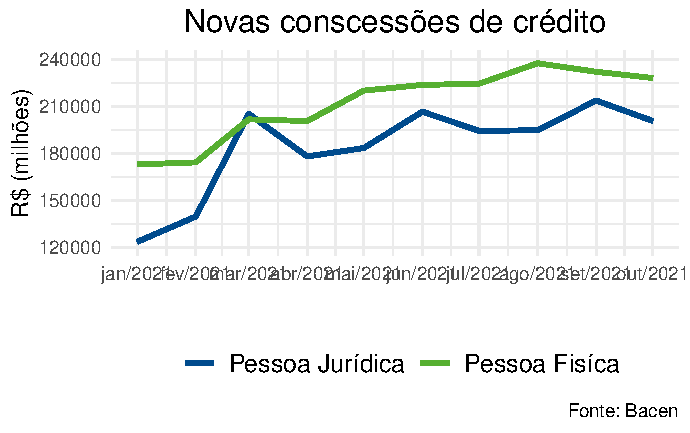
\includegraphics{credito_files/figure-latex/novas concessoes-1} \end{center}

A concessão de crédito livre às empresas foi de 189,8 bilhões, com queda
de 2,2\% em relação ao mês anterior, sem ajuste sazonal e aumento de
13,5\% no acumulado em doze meses. As modalidades de antecipação de
faturas de cartão de crédito (5,5\%), capital de giro com prazo superior
a 365 dias (0,9\%) e financiamento às exportações (3,0\%) se destacam.
Em relação a concessão de crédito direcionado, destinadas principalmente
ao investimento de médio e longo prazos aos setores imobiliário, rural e
de infraestrutura, atingiu R\$ 34,4 bilhões em outubro, com retração de
44,4\% sem ajuste sazonal e retração interanual de 27,2\%.

Para as pessoas físicas, a concessão de crédito livre foi de
R\(193,8 no mês de outubro, com queda de 0,2% em relação ao mês anterior, sem ajuste sazonal. Em se tratando do crédito direcionado o valor foi de R
\) 34,4 bilhões em outubro, queda de 9,3\% sem ajuste sazonal, em
relação ao mês anterior e alta de 42,4\% na comparação interanual.
\newpage

\section{O Indicador de Custo do Crédito (ICC) e Inadimplência} 
 \vspace{0,20cm}

O Indicador de Custo do Crédito (ICC), atingiu 18,0\% a.a., elevando-se
0,3 p.p. no mês e 0,8 p.p. na comparação com outubro de 2020. No crédito
livre não rotativo, o ICC situou-se em 23,7\% a.a., variações de 0,4
p.p. em outubro (0,8 p.p. na comparação interanual). O spread geral do
ICC situou-se em 12,3 p.p. (+0,1 p.p. no mês e +0,2p.p. na comparação
interanual).

A inadimplência total permaneceu estável em outubro, no patamar de
2,3\%, essa taxa se mantem por seis meses consecutivos. Por segmento, o
crédito livre registrou estabilidade neste indicador em 3,0\% do total
da carteira, enquanto nas operações direcionadas a inadimplência
apresentou redução de 0,1 p.p. ao atingir 1,2\%.
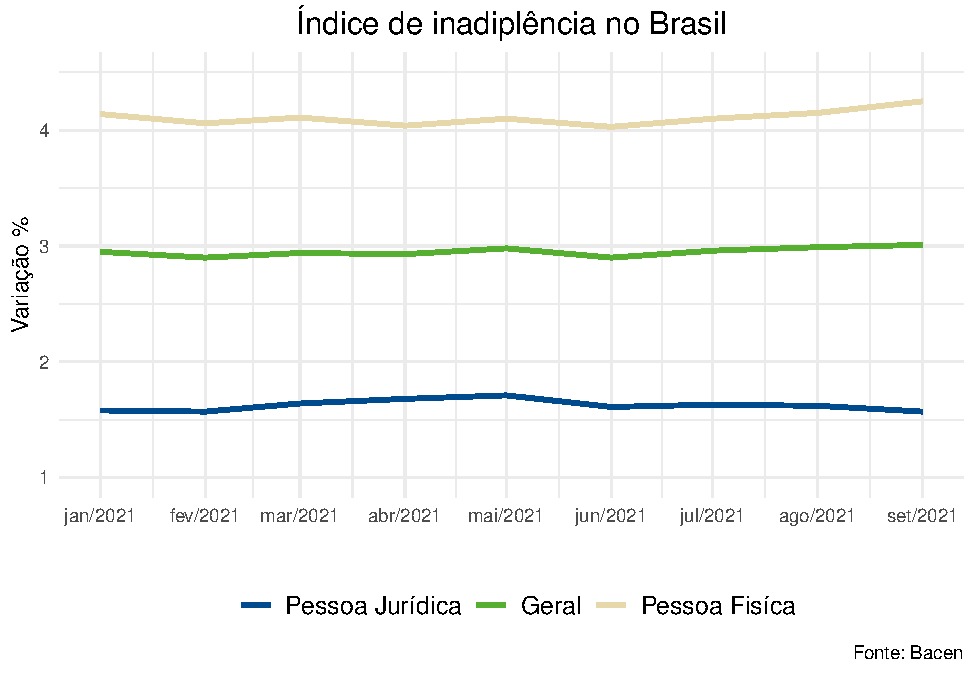
\includegraphics{credito_files/figure-latex/inadiplencia-1.pdf}


\end{document}
